\documentclass[12pt, a4paper]{article}

\usepackage[spanish]{babel}
\usepackage{amsmath}
\usepackage[labelfont=bf]{caption}


\usepackage{hyperref}
\hypersetup{
    colorlinks,
    citecolor={red!50!black},
    linkcolor={blue!50!black},
    urlcolor={blue!80!black}
}

\usepackage{mathtools}
\usepackage{multicol}
% \usepackage{esvect}
\usepackage{siunitx}
\usepackage{physics}
\AtBeginDocument{\RenewCommandCopy{\qty}{\SI}}
\usepackage{parskip}
\usepackage{xcolor}
% Circuitikz
\usepackage[american, RPvoltages]{circuitikz}
\usetikzlibrary{calc}
\usetikzlibrary{patterns}
\ctikzset{quadpoles/fourport/height=3}
\ctikzset{quadpoles/fourport/width=1.5}
% \ctikzset{bipoles/length=0.8cm}
% \ctikzset{bipoles/diode/height=.375}
% \ctikzset{bipoles/diode/width=.3}
% \ctikzset{tripoles/thyristor/height=.8}
% \ctikzset{tripoles/thyristor/width=1}
% \ctikzset{bipoles/vsourceam/height/.initial=.7}
% \ctikzset{bipoles/vsourceam/width/.initial=.7}
% \tikzstyle{every node}=[font=\small]
% \tikzstyle{every path}=[line width=0.8pt,line cap=round,line join=round]


% Bold vectors
\renewcommand{\vec}[1]{\mathbf{#1}}
\makeatletter
\newcommand{\vv}[2][]{
    \@ifempty{#1}{\vec{#2}}{\vec{#2}_{#1}}
}
\makeatother

\title{Apuntes de Sistemas Electroacústicos}
\author{Javier Rodrigo López}
\date{\today}
 

%%%%%%%%%%%%%%%%%%%%%%%%%%%%%%%%%%%%%%%%%%%%%%%%%%%%%
\begin{document}
% \renewcommand{\arraystretch}{1.2}
\maketitle

% Table of contents
\tableofcontents

\newpage
\section*{Introducción}

\section{Altavoces}

\subsection{Introducción al altavoz electrodinámico}


Un altavoz se compone de varios elementos:

\begin{itemize}
  \item Imán.
  \item Bobina.
  \item Membrana, cono o diafragma.
  \item Bornas de conexión (entre la membrana y la bobina).
\end{itemize}

A bajas frecuencias se puede aproximar al comportamiento de un pistón, pero a altas frecuencias pueden aparecer resonancias.

\subsubsection{Sección eléctrica}

\begin{figure}
  \centering
  \begin{circuitikz}[scale=0.8, transform shape]
    \draw (0,0) node[fourport, anchor=port1] (A) {};
    \coordinate (A1) at (A.port1);
    \coordinate (A4) at (A.port4);

    \draw (3,0) node[fourport, anchor=port1] (B) {};

    \draw (6,0) node[fourport, anchor=port1] (C) {};
    \draw (9,0) node[fourport, anchor=port1] (D) {};
    \draw (12,0) node[fourport, anchor=port1] (E) {};


    \draw (A1) to ++(-2,0) node(corner){} to[sV, v=$ $, l_=$e_g$] (corner|-A4) to[R, l=$R_e$] (A4);

    % Líneas de abajo
    \draw (A.port2) to (B.port1);
    \draw (B.port2) to (C.port1);
    \draw (C.port2) to (D.port1);
    \draw (D.port2) to (E.port1);
    % Líneas de arriba
    \draw (A.port3) to (B.port4);
    \draw (B.port3) to (C.port4);
    \draw (C.port3) to (D.port4);
    \draw (D.port3) to (E.port4);

    % Draw labels on center of fourports
    \node[align=center] at (A.center) {Sección\\eléctrica};
    \node[align=center] at (B.center) {Sección\\electro-\\mecánica};
    \node[align=center] at (C.center) {Sección\\mecánica};
    \node[align=center] at (D.center) {Sección\\mecánico-\\acústica};
    \node[align=center] at (E.center) {Sección\\acústica};

    % Draw underbrace
    \node[align=center] at (-1.1,-0.5) (hola) {$\underbrace{\phantom{holaaaaaa}}_{\text{Amplificador}}$};

  \end{circuitikz}
  \caption{Modelo de altavoz electrodinámico}
\end{figure}

\subsubsection{Sección de conversión electromećanica}

\subsubsection{Sección mecánica}

Las partes mécanicas del altavoz son la membrana y la araña (suspensión). En términos de mecánica, este sistema es equivalente a un pistón, un muelle y una masa. TODO Copiar el diagrama del cuaderno.

\begin{equation} \label{eq:ley_hooke}
  F = -kz
\end{equation}

\begin{equation} \label{eq:amortiguamiento}
  F = -d \dv{z}{t}
\end{equation}

Donde $d$ es la disipación de energía por rozamiento.

\begin{equation} \label{eq:masa}
  F = m \dv[2]{z}{t}
\end{equation}

\begin{equation} \label{eq:ecuacion_seccion_mecanica}
  F - k z - d \dv{z}{t} = m \dv[2]{z}{t}
\end{equation}

\begin{equation} \label{eq:ecuacion_seccion_mecanica_2}
  F = kz + d \dv{z}{t} + m \dv[2]{z}{t}
\end{equation}

\subsubsection{Sección de conversión mecánico-acústica}

Para hallar la impedancia de radiación, recordamos que una impedancia es la relación entre tensión y corriente. En nuestro modelo, la tensión se relaciona con la velocidad y la corriente con la fuerza. Por lo tanto, la impedancia de radiación es la relación entre la velocidad de la membrana y la fuerza que se ejerce sobre ella.

La impedancia acústica mide cuánto se está oponiendo el medio acústico (aire) al movimiento del pistón. El pistón comprime y expande el aire y genera una variación de la presión.

\begin{equation} \label{eq:incremento_presion}
  \dd p_1 = j\omega\rho_0 v_z d S_1 \frac{e^{-jkr_1}}{2\pi r_1}
\end{equation}

Una región 1 del pistón genera una fuerza sobre otra región 2 del pistón de la siguiente manera:
\begin{equation} \label{eq:presion_de_1_sobre_2}
  \dd f_{1,2} = j\omega \rho_0 v_z d S_1 \frac{e^{-jkr_1}}{2\pi r_1} \dd S_2
\end{equation}

\begin{equation} \label{eq:presion_de_2_sobre_1}
  F = \frac{j\omega \rho_0 v_z}{2\pi} \int_{S_1} \int_{S_2} \frac{e^{-jkr_{1,2}}}{r_{1,2}} \dd S_1 \dd S_2
\end{equation}

La solución de esta ecuación es:

\begin{equation} \label{eq:impedancia_piston}
  Z_{ac} = \frac{F}{v_z} = \pi a^2 \rho_0 c \left[ \left( 1 - \frac{J_1 (2ka)}{ka}  \right) + j \left( \frac{H_1 (2ka)}{ka} \right)\right]
\end{equation}

Donde $J_1$ y $H_1$ son la función de Bessel de primer tipo y orden 1 y la función de Struve de primer tipo y orden 1, respectivamente. Podemos ver la representación de la impedancia de radiación en la \autoref{fig:impedancia_radiacion}.

\begin{figure}[htp]
  \centering
  \caption{Impedancia de radiación acústica de un pistón}
  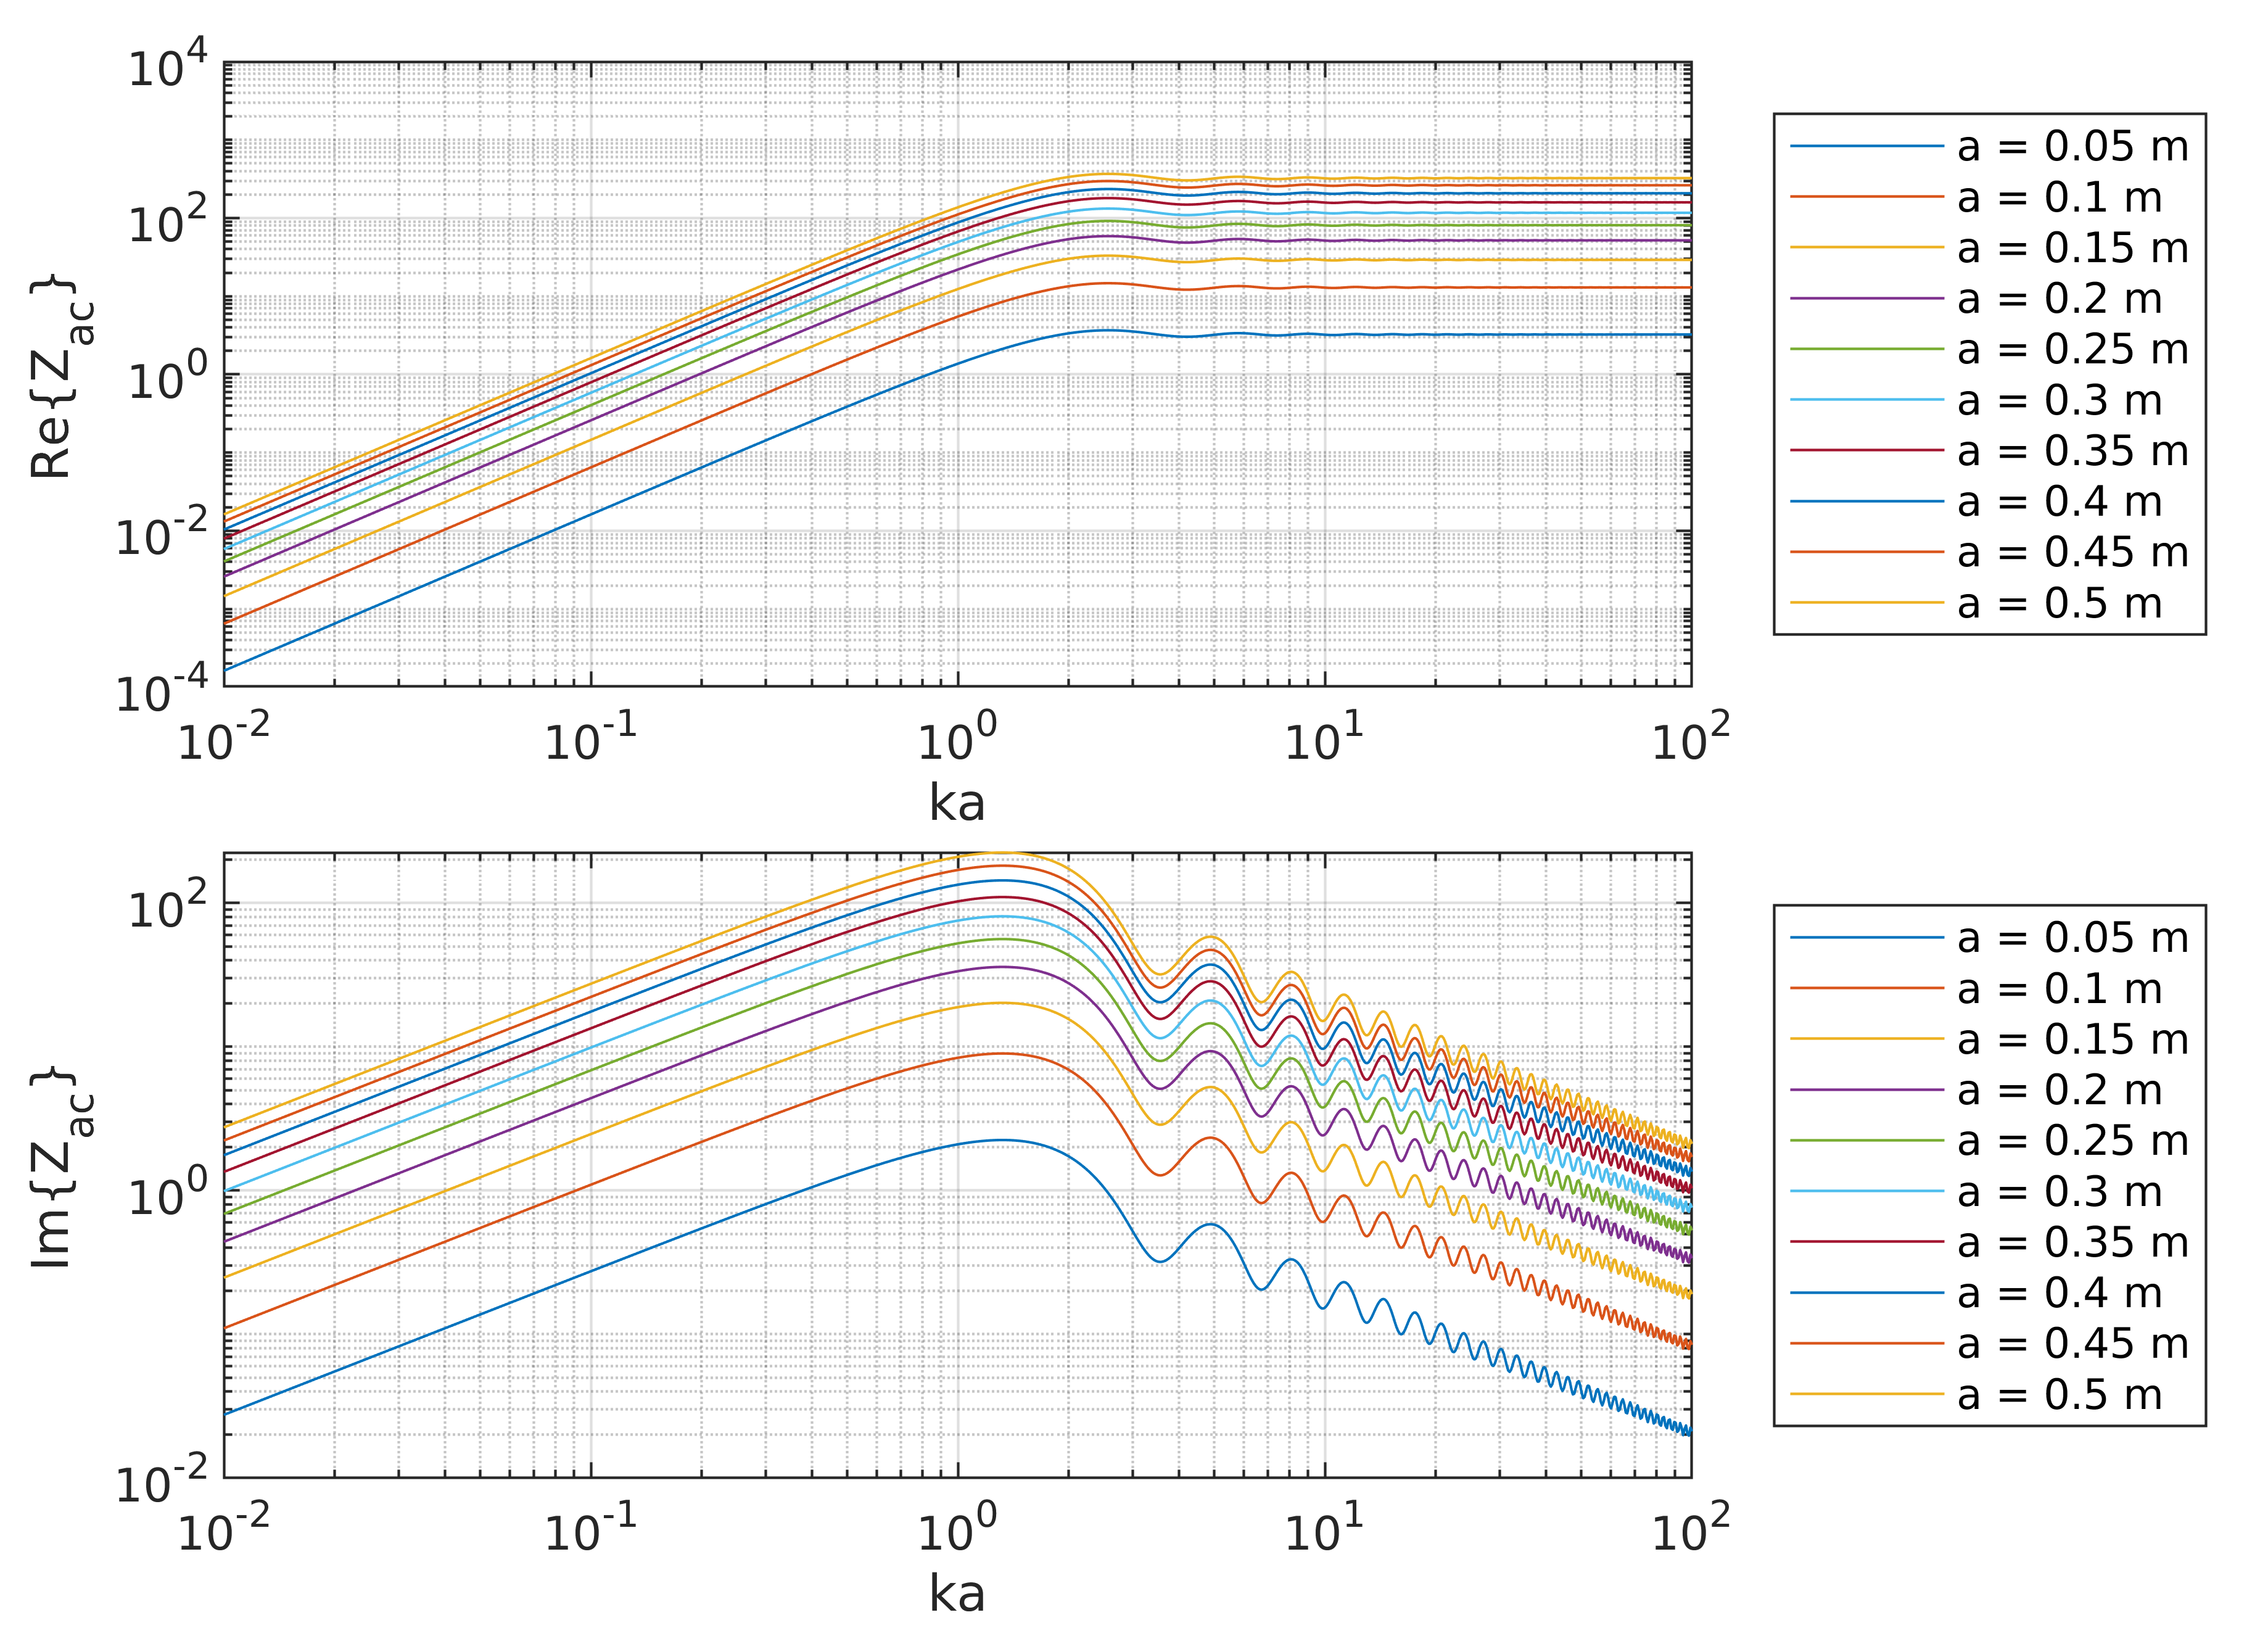
\includegraphics[width=\linewidth]{images/acoustic_radiation_impedance.png}
  \label{fig:impedancia_radiacion}
\end{figure}



\subsubsection{Modelo completo del altavoz}

\begin{figure}[htp]
  \centering
  \caption{Modelo eléctrico completo del altavoz}
  \begin{circuitikz}[scale=0.9, transform shape]
    \draw (0,0) to[sV, v=$e_g'$] ++(0,3) to[R=$R_E'$] ++(2,0) to[L=$L_E'$] ++(2,0) to [R=$R_{MS}$, *-*] ++(0,-3) to[short] (0,0);
    \draw (4,3) to[short] ++(1.5,0) to[L=$C_{MS}$, *-*] ++(0,-3) to[short] ++(-1.5,0);
    \draw (5.5,3) to[short] ++(1.5,0) to[C=$M_{MS}$, *-*] ++(0,-3) to[short] ++(-1.5,0);
    \draw (7,3) to[R=$R_{AP-LF}$, -*] ++(3, 0) to[short] ++(0,1) to[R=$R_{AP-HF} - R_{AP-LF}$] ++(2,0) to[short, -*] ++(0,-1)  to[short] ++(1,0) to[C=$M_{AP}$] ++(0,-3) to[short] ++(-6,0);
    \draw (10,3) to[short] ++(0,-1) to[L=$L_{AP}$] ++(2,0) to[short] ++(0,1)
    ;
  \end{circuitikz}
  \label{fig:modelo_completo_altavoz}
\end{figure}

\begin{align*}
  e'_g & = \frac{e_g}{Bl}                      & R_{MS} & = \frac{1}{d} & R_{AP-LF} & = \frac{1}{2} \cdot \frac{9\pi}{\rho_0ca^2}  \\
  R'_E & = \frac{R_g+R_E}{\left( Bl \right)^2} & C_{MS} & = \frac{1}{k} & R_{AP-HF} & = \frac{1}{2} \cdot \frac{1}{\rho_0c\pi a^2} \\
  L'_E & = \frac{L_E}{\left( Bl \right)^2}     & M_{MS} & = m           & M_{AP}    & = 2 \cdot \frac{8}{3} \rho_0 a^3             \\
\end{align*}

A \textbf{baja frecuencia}, la impedancia de radiación es fundamentalmente capacitiva.

Tras calcular la $Z_{\text{eq}}$ (ver cuaderno), podemos ver que el sistema se comporta como un filtro paso banda. La función de transferencia del sistema queda así:
\begin{equation} \label{eq:funcion_transferencia_altavoz_LF}
  H_{LF}(s) = \frac{H_0 s }{s^2 + \frac{\omega s }{Q } + \omega_s^2}
\end{equation}

\begin{equation} \label{eq:impedancia_altavoz_LF}
  Z_{LF}(s) = \frac{\frac{1}{C_{\text{eq}}s}}{s^2 + \frac{1}{C _{\textnormal{eq}R_{MS}}}s + \frac{1}{C_{\text{eq}}C_{MS}}}
\end{equation}

\begin{equation} \label{eq:f_res_LF}
  \omega_s = \frac{1}{\sqrt{C_{\text{eq}}C_{MS}}}
\end{equation}

Como $\frac{1}{Q _{\text{eq}}} = \frac{\omega_s}{Q}$, entonces:
\begin{equation} \label{eq:factor_calidad}
  Q = \omega_s R_{MS} C _{\text{eq}} = R_{MS} \sqrt{\frac{C _{\text{eq}}}{C_{MS}}}
\end{equation}

Donde $Q$ es el factor de calidad del sistema correspondiente a la parte mecánica y acústica.

La impedancia máxima que ve el sistema es $R_d$ a la frecuencia de resonancia.

La impedancia eléctrica total será:
\begin{equation} \label{eq:impedancia_electrica}
  Z_E = R_E + \frac{\left( Bl \right)^2 \frac{1}{C _{\text{eq}}}s}{s^2 + \frac{1}{R_{MS}C _{\text{eq}}}s + \frac{1}{C _{\text{eq}}C_{MS}}}
\end{equation}

Este sistema, que tiene en cuenta también la parte eléctrica del altavoz, tendrá un factor de calidad diferente que llamaremos \textbf{factor de calidad total} $Q_t$ y que será:
\begin{equation} \label{eq:factor_calidad_total}
  Q_t = ?
\end{equation}

\textit{Correcciones que ha hecho el profe en clase el día lunes 30 de septiembre}

\[ \frac{v_z}{e_g} = \frac{Z_{MS}}{R_E' + Z_{MS}} = \frac{\frac{Z_0}{R_E'}s}{s^2 + \left( \frac{\omega_s}{Q_{MS}} + \frac{Z_0}{R_E'} \right) s + \omega_s^2} \]

Donde el término del denominador que acompaña a $s$ resulta que es $\frac{\omega_s}{Q_T}$. Es decir:

\[ \frac{\omega_s}{Q_T} = \frac{\omega_s}{Q_{MS}} + \frac{Z_0}{R_E'} \]

Valores realistas:

\begin{align*}
  R_E    & = 7.5                 \\
  L_E    & = 300 \times 10^{-6}  \\
  M_{MS} & = 0.03                \\
  R_{MS} & = \frac{1}{6}         \\
  C_{MS} & = 6 \times 10^{-5}    \\
  C_{AP} & = 21.3 \times 10^{-3} \\
  R_{AP} & = 17.3 \times 10^{-3} \\
\end{align*}


\begin{figure}[htp]
  \centering
  \caption{Modelo del altavoz a alta frecuencia}
  \begin{circuitikz}
    \draw (0,0) to[sV, v=$e_g'$]  ++(0, 3) to[L=$L_E'$, -*] ++(3,0) node(n1){} to[short, -*] ++(2,0) node(n2){} to[R=$R_{AP-HF}$] ++(3,0) to[short] ++(0,-3) to[short, -*] ++(-3,0) node(n3){} to[C, l_=$M_{MS}$, -|] (n2.center);
    \draw (n3.center) to[short, -*] ++(-2,0) node(n4){} to[R=$R_{MS}$] (n1.center);
    \draw (n4.center) to[short] (0,0);
    \draw (n4) to[open] ++(1,0) node[ground]{};
  \end{circuitikz}
  \label{fig:altavoz_HF}
\end{figure}

A \textbf{alta frecuencia}, el sistema depende de características mecánicas y eléctricas.

\[ Z_{MS} = \left( \frac{1}{R_{MS}} + \frac{1}{R_{AP}} + s M_{MS}  \right) ^{-1} \]

\[ \frac{v_z}{e_g} = \frac{Z_{MS}}{L_E's + Z_{MS}} = \frac{1}{1 + L_E' \left( \frac{1}{R_{MS}} + \frac{1}{R_{AP}} + sM_{MS} \right) s }  \]

\textbf{RESUMEN.}
\begin{enumerate}
  \item A \textbf{baja frecuencia}, el efecto dominante es la característica mecánica (la rigidez del muelle).
  \item Existe una \textbf{resonancia mecánica} que depende de las pérdidas (resistencias y amortiguamiento) y el campo magnético.
  \item A \textbf{frecuencias medias} la respuesta es constante y dominada por la masa.
  \item Existe una \textbf{resonancia electromecánica} determinada por la bobina ya que almacena bastante energía.
  \item A \textbf{alta frecuencia} la bobina almacena mucha energía y aumentar la frecuencia (velocidad del altavoz) cuesta mucho.
\end{enumerate}

TODO: Análisis de matlab de diapositiva 15

TODO: Análisis de matlab de diapositiva 16. Nota. En esta diapositiva no independica la potencia disipada en $Z_E$ y $Z_{MS}$. Se podría hacer para ver cómo afecta.

\subsubsection{Transferencia de potencia}

La respuesta de potencia define el \textbf{ancho de banda} del altavoz.

\begin{align*}
  \overline{P_g}               & = \frac{1}{2} \Re \left\lbrace E_g I_g^* \right\rbrace = \frac{1}{2} \Re \left\lbrace E_g \frac{E_g^*}{R_g + Z^*_{\text{total}}} \right\rbrace                              \\
  \overline{P _{\text{total}}} & = \frac{1}{2} \Re \left\lbrace V _{\text{total}} I_g^* \right\rbrace = \frac{1}{2} \Re \left\lbrace E_g \frac{Z_{\text{total}}}{R_g + Z_{\text{total}}} I_g^* \right\rbrace
\end{align*}

\subsubsection{Diagrama de radiación}

¿Cómo contribuye cada punto $\left( x', y', z' \right)$ del pistón a la presión en un punto del espacio $\left( x, y, z \right)$?

Primero se supone que el punto $\left( x', y', z' \right)$ se ubica en \textit{campo lejano}. Es decir, las dimensiones del altavoz son mucho más pequeñas que la distancia del altavoz al punto:

\begin{equation} \label{eq:campo_lejano}
  r \geq 2 \frac{\left( 2a \right)^2}{\lambda} = \frac{8a^2}{\lambda}
\end{equation}

Sin entrar en detalles, la solución es:

\begin{equation} \label{eq:presion_punto}
  \abs{p(r,\theta)} \propto \frac{2 J_1(ka \sen \theta)}{ka \sen \theta}
\end{equation}

Donde $J_1$ es la función de Bessel de primer tipo y orden 1. Las conclusiones a las que podemos llegar tras ver esta solución:

\begin{itemize}
  \item La presión depende del ángulo de radiación $\theta$.
  \item La presión es máxima en el eje del altavoz.
  \item Como $k= \frac{2\pi}{\lambda}$, la presión depende de la relación $\frac{a}{\lambda}$. En otras palabras, de la frecuencia.
  \item Para altavoces de gran diámetro, el campo lejano se alcanza a distancias mayores. Por lo tanto, es común que esta aproximación no sirva a distancias cortas para altavoces de gran tamaño.
\end{itemize}

VER GRÁFICA DIAPOSITIVA 18. El diagrama de radiación depende del radio del altavoz. La radiación de un altavoz puede ser adecuada en ciertas frecuencias (que para cualquier ángulo $\theta$ la presión sea máxima) o muy mala y que existan cancelaciones de presión para ciertos ángulos.

Cuando el altavoz no opera en campo lejano, los cálculos son mucho más complejos y solo se pueden encontran soluciones sencillas en el eje $\theta=0$. Algunas frecuencias se anulan completamente, y a distancias en torno a $r=\lambda$ en ocasiones se producen mínimos. Esto no es un problema tan grande si se trata de frecuencias bajas.

\subsection{Parámetros de altavoces}
\subsubsection{Respuesta en frecuencia}

La respuesta se da en términos de la presión sonora (SPL), siendo la presión de referencia $p _{\text{ref}} = \qty{20}{\micro\pascal}$ y definida para unas ciertas condiciones:
\begin{itemize}
  \item Señal de entrada con potencia de \qty{1}{\watt}.
  \item Distancia al centro acústico del altavoz de \qty{1}{\meter}.
  \item Medido en el eje del altavoz ($\theta = \qty{0}{\degree}$).
\end{itemize}

Señales de entrada para su medida:
\begin{itemize}
  \item Barrido de tonos de amplitud constante. La duración del barrido determinará la resolución en frecuencia.
  \item Señales con ancho de banda con un tercio de octava.
\end{itemize}

\subsubsection{Impedancia}

Es común que los altavoces sean autoamplificados, es decir, que integran el amplificador eléctrico en la propia caja del altavoz. En este tipo de altavoces no es común ni necesario que den datos sobre la impedancia del altavoz.

Típicamente se da el módulo (omitiendo la fase) $\abs{Z _{\text{total}}(f)}$. Se suele ofrecer una \textbf{impedancia nominal} definida a menudo como el valor mínimo de impedancia obtenido a partir de la frecuencia de resonancia.

Orientativamente:

\begin{equation} \label{eq:impedancia_nominal}
  Z _n \leq \frac{\min \abs{ Z _{\text{total}}(f)} }{0.8}
\end{equation}

Valores típicos de la impedancia nominal suelen ser \qty{4}{\ohm}, \qty{8}{\ohm} y \qty{16}{\ohm}. A veces podemos encontrar otras.

\subsubsection{Sensibilidad}

Cualquiera de las siguientes definiciones es válida:
\begin{itemize}
  \item \color{blue} La sensibilidad es el valor medio de presión sonora en el rango de frecuencias del altavoz a una distancia de \qty{1}{\meter} en el eje con una potencia eléctrica fija de \qty{1}{\watt}. \color{black}
  \item \color{blue} La sensibilidad del altavoz se define como el nivel de presión sonora radiada por el altavoz cuando se le excita con una potencia de \qty{1}{\watt}, sobre la impedancia nominal, a \qty{1}{\meter} de
        distancia y en el eje de máxima radiación. \color{black}
\end{itemize}



La tensión en bornes del altavoz se puede obtener como:
\[ P = V  I = \frac{V^2}{Z_N} \qquad \Longrightarrow \qquad V = \sqrt{P   Z_N} \]

Si la potencia o la distancia cambian, que puede pasar si las condiciones de medida no pueden cumplirse\footnote{Para altavoces de gran diámetro, es posible que la distancia de \qty{1}{\meter} se encuentre en campo cercano. Para medir la sensibilidad se escoge entonces una distancia mayor.}, se aplica una corrección:

TODO: Añadir ecuación de corrección

\subsubsection{Potencia}
\subsubsection{Distorsión}
\subsubsection{Directividad}
\subsubsection{Parámetros de Thielle-Small}

\begin{itemize}
  \item \textbf{Frecuencia de resonancia mecánica:} $f_s$
  \item \textbf{Superficie efectiva del diagrama} $S_d$
  \item \textbf{Resistencia de la bobina en corriente continua} $R_e$
  \item \textbf{Factor de calidad total}\footnote{Recordatorio: El factor de calidad (a veces llamado factor de sobrecarga) se puede calcular como $Q= \frac{\omega_0}{\Delta \omega} = 2\pi \frac{\text{Energía almacenada}}{\text{Energía disipada por ciclo}}$.} $Q_t$
  \item \textbf{Factor de calidad eléctrico} $Q_{ES}$
  \item \textbf{Factor de calidad mecánico} $Q_{MS}$
        \[ Q_t = \frac{Q_{ES}Q_{MS}}{Q_{ES} + Q_{MS}} \]
  \item \textbf{Volumen de aire equivalente a la ductilidad de suspensión:} $V_{AS} = \rho_0c^2S_D^2C_{MS}$
  \item \textbf{Desplazamiento máximo del cono con respecto al reposo:} $X_{\text{max}}$
\end{itemize}

TODO: Añadir resolución del T1-Problema 1
TODO: Añadir resolución del T1-Problema 2

\subsection{Altavoces en caja cerrada}

\newpage
\section{Filtros de cruce}

\subsection{Introducción}

\subsection{Filtros pasivos}

Los filtros se definen por dos parámetros: la \textbf{frecuencia de resonancia} $\omega _r$ y el \textbf{factor de calidad} $Q$.

Los \textbf{filtros de Butterworth} se caracterizan por no presentar oscilaciones (\textbf{rizado}) en la banda de paso.

Cuando $Q>\frac{1}{\sqrt{2}}$ se considera que el filtro es \textbf{resonante} (aparece un pequeño aumento de la amplitud en la frecuencia de cortes).

TODO Añadir gráficas de un filtro para diferentes valores de $Q$


\subsubsection{Filtros de segundo orden}

Para filtros de cruce, los valores de $Q$ utilizados son típicamente $Q=\frac{1}{2}$, que se corresponde con un amortiguamiento crítico. Además, $\omega_l = \omega_{m1}$ y $\omega_h = \omega_{m2}$.

Para conseguir que la respuesta sea lo más plana posible, se debe definir la frecuencia de corte a \qty{-6}{\dB}.

\subsection{Ajuste de niveles}

Cuando una caja tiene varias vías, significa que tenemos altavoces diferentes con parámetros diferentes. El objetivo del ajuste de niveles es \textbf{igualar la sensibilidad} en las bandas de paso.

Al modificar $R _{\text{in}}$ se ve afectado $Q_{ES}$, sobre todo en el woofer. La corrección necesaria será:
\begin{equation} \label{eq:correccion_niveles}
  k _{\text{pad}} = 10^{\frac{S \left[ \unit{\volt} \text{ rel } p_0\right] _{\text{ref}} - \left[ \unit{\volt} \text{ rel } p_0 \right] }{20}}
\end{equation}

\subsection{Ecualización de alta frecuencia}

Recordamos que a alta frecuencia el altavoz no presenta un comportamiento resistivo. La bobina $L_E$ afectará a la respuesta. Para corregir esto, existen varias soluciones:
\begin{itemize}
  \item Integrar $L_E$ en el diseño del filtro de cruce.
  \item Situar la frecuencia de cruce por encima de la de resonancia de los altavoces (midranges y tweeters).
  \item Introducir un \textbf{ecualizador}.
\end{itemize}

La ecualización se tendrá que hacer con el objetivo de aplanar la zona de alta frecuencia y además aplanar la resonancia. TODO Mirar la diapositiva 17.

\subsection{Funciones de transferencia globales}

Al trabajar con una caja de tres vías, veremos que la respuesta en la sala será la combinación del efecto de los tres altavoces. En cada punto de la sala, se sumarán las amplitudes y por ello la fase con la que emite cada altavoz será muy importante. Por si no fuera poco, el filtro de cruce también afectará a la fase.

Decisiones a tomar:
\begin{itemize}
  \item Se debe elegir si sumar salidas con polaridad invertida.
  \item Se debe seleccionar $Q$ para lograr respuesta plana.
  \item Se decidirá si se usan filtros paso-todo para corregir la fase.
\end{itemize}


\end{document}